\subsection{Array}
\begin{frame}[fragile]
\frametitle{Array}
An array is stored as one piece in the memory.\\
Use an array if
\begin{itemize}
\item you need indexed or random access to elements
\item you know the number of elements which will be stored in the array
\item you need speed when iterating through all elements
\item memory is a concern (a linked list needs much more memory)
\end{itemize}
\end{frame}

\subsection{Linked List}
\begin{frame}[fragile]
\frametitle{Linked List}
In a linked list, all elements are distributed in the memory. An additional pointer
for each element is needed to store the location of the next element.\\
Use a linked list if
\begin{itemize}
\item you need constant time for insertions and deletions
\item you do not know how many elements will be stored in the list
\item you do not need random access
\end{itemize}
\end{frame}

\begin{frame}[fragile]
\frametitle{Linked List}
A linked list in the memory:\\
\vspace{1mm}
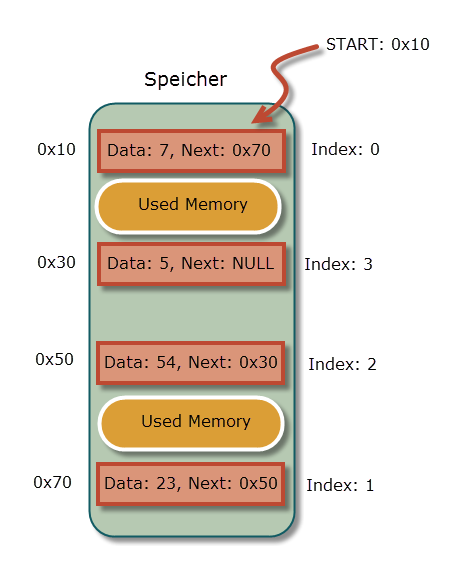
\includegraphics[scale=0.35]{img/linkedlist.png}
\end{frame}

\begin{frame}[fragile]
\frametitle{Linked List}
Insert into a linked list:\\
\vspace{1mm}
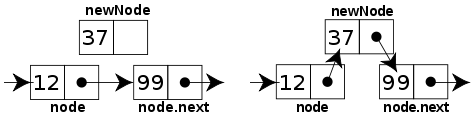
\includegraphics[scale=0.3]{img/linkedlist_insert2.png}\\
\vspace{5mm}
Delete from a linked list:\\
\vspace{1mm}
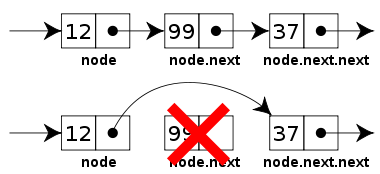
\includegraphics[scale=0.3]{img/linkedlist_remove2.png}
\end{frame}

\begin{frame}[fragile]
\frametitle{Array, Linked List}
\begin{exercise}
Create a abstract base class \verb|Container| which contains the most
important operations to read and write data into a container.
\end{exercise}
\begin{exercise}
Create 2 sub classes of the class \verb|Container|. Implement all abstract
methods (one class is based on an array, the other one on a linked list).
\end{exercise}
\end{frame}

\subsection{Stack}
\begin{frame}[fragile]
\frametitle{Stack}
A stack is a \emph{LIFO} (last in, first out) data type that serves as a collection
of elements with two principal operations: push and pop.\\
push adds an element to the collection, pop removes the last element that was added.\\
\vspace{1mm}
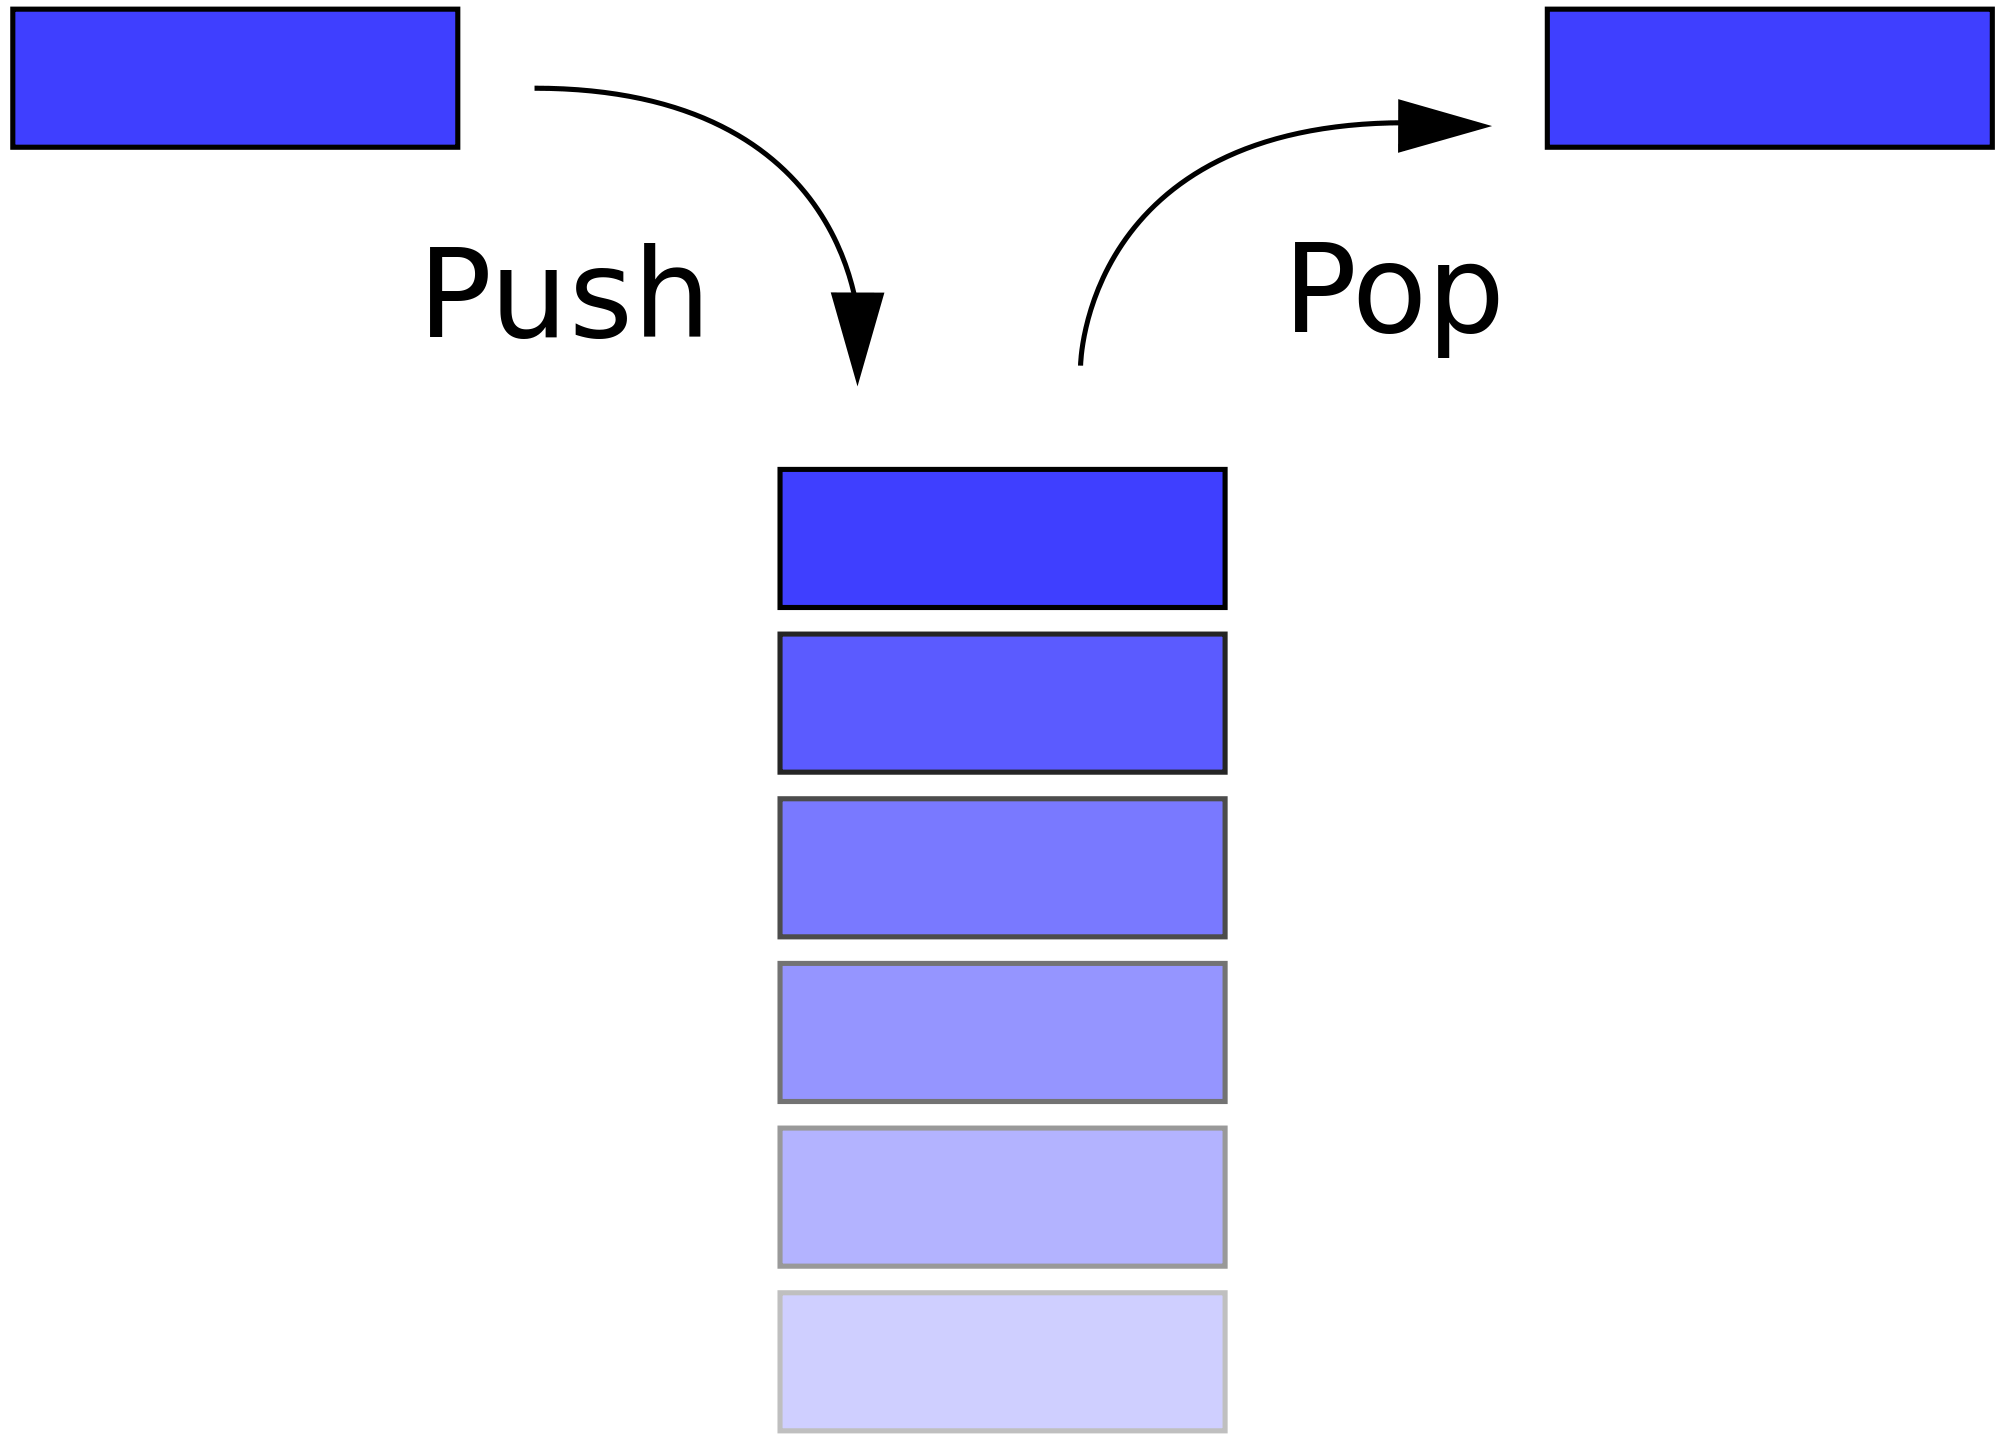
\includegraphics[scale=0.06]{img/stack.png}
\end{frame}

\begin{frame}[fragile]
\frametitle{Stack}
{\tiny
\begin{lstlisting}
class Stack {
private:
  int *values; // array based stack
  int maxNumberOfElement;
  int index;
private:
  Stack();
  Stack(const Stack & obj);
  Stack operator= (const Stack & obj);
  virtual ~Stack();
  bool pop(int & value);
  bool push(int value);
  bool top(int & value);
  int size();
  bool isEmpty();
};
\end{lstlisting}
}
\end{frame}

\subsection{Queue}
\begin{frame}[fragile]
\frametitle{Queue}
A queue is a \emph{FIFO} (first in, first out) data type that serves as a collection
of elements with two principal operations: enqueue and dequeue.\\
enque adds an element to the collection, deque removes the first element that was added.\\
\vspace{1mm}
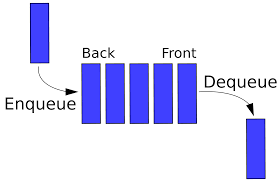
\includegraphics[scale=0.3]{img/queue.png}
\end{frame}

\begin{frame}[fragile]
\frametitle{Queue}
{\tiny
\begin{lstlisting}
class Queue {
private:
  Stack values; // stack based queue
private:
  Queue();
  Queue(const Stack & obj);
  Queue operator= (const Queue & obj);
  virtual ~Queue();
  bool deque(int & value);
  bool enque(int value);
  bool front(int & value);
  bool back(int & value);
  int size();
  bool isEmpty();
};
\end{lstlisting}
}
\end{frame}